\section{Auswertung}
\label{sec:Auswertung}

\subsection{Ausmessung des Acryl-Blocks mittels A-Scan}

Die Ausmessung des Blocks via Schieblehre und A-Scan führt zu den Daten, welche in Tabelle \ref{table:1} dargestellt sind.
\begin{table}
    \centering
    \caption{Messdaten zur Bestimmung der Ablenkung im B-Feld.}
    \label{table:A2}
    \sisetup{parse-numbers=false}
    \begin{tabular}{
	S[table-format=1.2]
	S[table-format=1.2]
	S[table-format=1.2]
	S[table-format=1.2]
	S[table-format=1.2]
	S[table-format=1.2]
	}
	\toprule
	{$D \:/\: \text{in}$}		& {$I_1 \:/\: \si{\ampere}$}		& 
	{$I_2 \:/\: \si{\ampere}$}		& {$I_3 \:/\: \si{\ampere}$}		& 
	{$I_4 \:/\: \si{\ampere}$}		& {$I_5 \:/\: \si{\ampere}$}		\\ 
	\midrule
    0.00 & 0.00 & 0.00 & 0.00 & 0.00 & 0.00 \\
0.25 & 0.28 & 0.30 & 0.32 & 0.35 & 0.40 \\
0.50 & 0.58 & 0.64 & 0.69 & 0.74 & 0.81 \\
0.75 & 0.89 & 1.00 & 1.07 & 1.14 & 1.25 \\
1.00 & 1.19 & 1.34 & 1.44 & 1.56 & 1.66 \\
1.25 & 1.52 & 1.68 & 1.81 & 1.94 & 2.09 \\
1.50 & 1.84 & 2.20 & 2.20 & 2.34 & 1.51 \\
1.75 & 2.18 & 2.39 & 2.58 & 2.75 & 2.94 \\
2.00 & 2.49 & 2.73 & 2.95 & /    & /    \\

    \bottomrule
    \end{tabular}
    \end{table}

Dabei ist anzumerken, dass der tatsächliche Abstand der beiden letzten Fehlstellen $\Delta D = \SI{1.8}{\milli\metre}$ entspricht.
Die Messung übergibt einen Abstand von $\Delta D = \SI{1.7}{\milli\metre}$.
Folglich besitzt der A-Scan eine minimale Auflösung von etwa $\SI{1.7}{\milli\metre}$.\\
Zur Berechnung wird eine Phasengeschwindigkeit von $\SI{2730}{\metre\per\second}$ verwendet. \cite{schall}

\subsection{Ausmessung des Acryl-Blocks mittels B-Scan}
Das Ergebnis des B-Scans von oben ist in Abbildung \ref{figure:1} wiedergegeben; das des unteren in Abbildung \ref{figure:2}.

\begin{figure}[H]
  \centering
  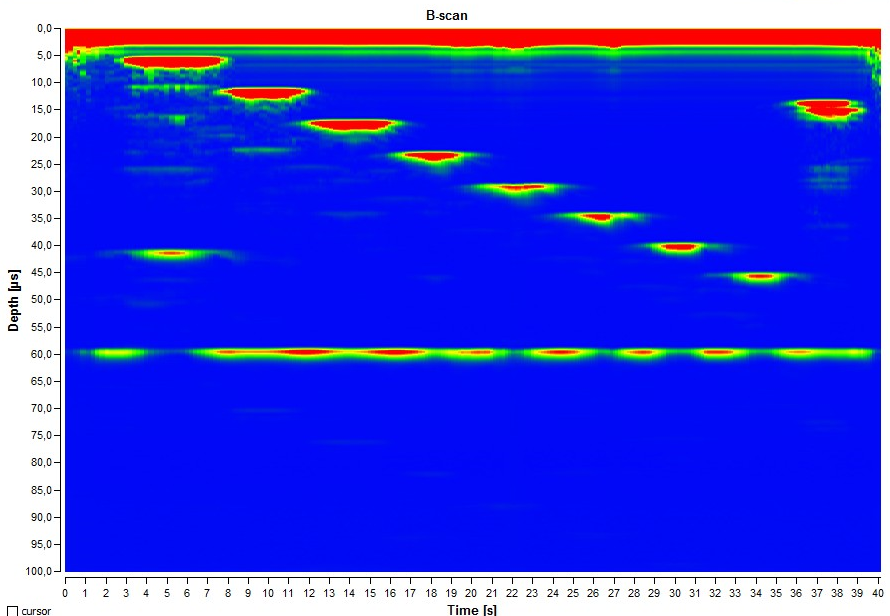
\includegraphics[height=7.5cm]{messdaten/b_oben.png}
  \caption{Ergebnis des B-Scans von oben.}
  \label{figure:1}
\end{figure}

\begin{figure}[H]
  \centering
  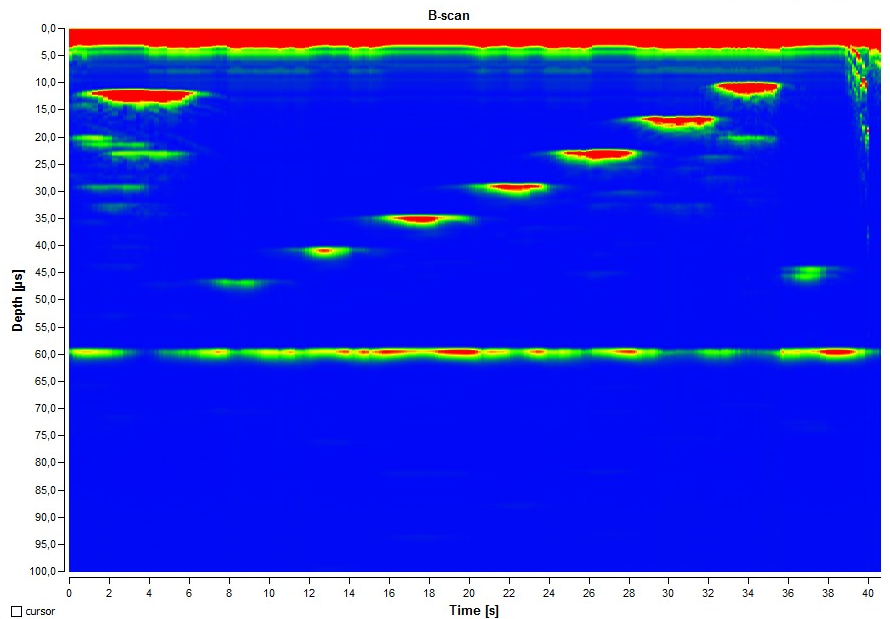
\includegraphics[height=7.5cm]{messdaten/b_unten.png}
  \caption{Ergebnis des B-Scans von unten.}
  \label{figure:2}
\end{figure}

Aus diesen beiden Grafiken ergeben sich die Messdaten aus Tabelle \ref{table:2}.
\begin{table}
    \centering
    \caption{Messdaten zur Bestimmung der Ablenkung im E-Feld.}
    \label{table:b}
    \sisetup{parse-numbers=false}
    \begin{tabular}{
	S[table-format=1.2]
	S[table-format=4.2]
	S[table-format=4.2]
	S[table-format=4.2]
	S[table-format=4.2]
	S[table-format=4.2]
	}
	\toprule
	{$D \:/\: \text{in}$}		& {$U_1 \:/\: \si{\volt}$}		&
	{$U_2 \:/\: \si{\volt}$}		& {$U_3 \:/\: \si{\volt}$}		&
	{$U_4 \:/\: \si{\volt}$}		& {$U_5 \:/\: \si{\volt}$}		\\
	\midrule
    0.00 & -8.55 & -11.09 & -13.35 & -14.23 & -17.43 \\
0.25 & -4.58 & -6.36  & -7.82  & -7.67  & -10.13 \\
0.50 & -1.10 & -1.87  & -1.96  & -1.06  & -2.40  \\
0.75 & 2.61  & 2.91   & 3.79   & 5.38   & 5.17   \\
1.00 & 6.18  & 7.59   & 8.92   & 11.67  & 12.58  \\
1.25 & 9.59  & 12.00  & 14.64  & 17.93  & 19.83  \\
1.50 & 13.26 & 16.60  & 20.09  & 24.32  & 27.00  \\
1.75 & 16.80 & 20.98  & 25.31  & 30.78  & 34.23  \\
2.00 & 20.40 & 25.35  & 30.81  & /      & /      \\

    \bottomrule
    \end{tabular}
    \end{table}

\\In der Diskussion werden die Ergebnisse aus A- und B-Scan verglichen.

\subsection{Untersuchung des Herzmodells}

Ausgangspunkt der Messung der Herzfrequenz und des Herzvolumens ist der TM-Scan aus Abbildung \ref{figure:3}.

\begin{figure}[H]
  \centering
  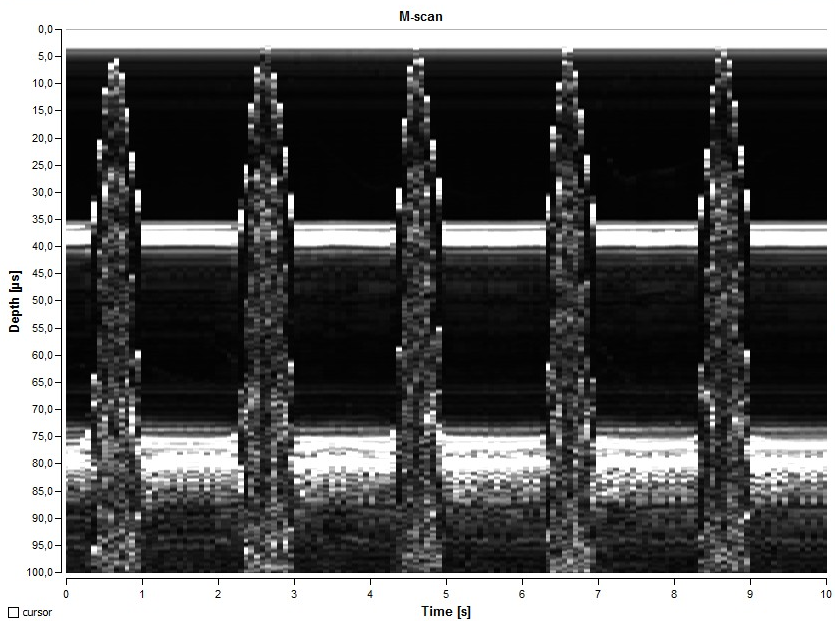
\includegraphics[height=9cm]{messdaten/herz.png}
  \caption{TM-Scan des schlagenden Herzmodells.}
  \label{figure:3}
\end{figure}

Dabei ergeben sich für die Amplituden die Werte
\begin{align*}
  A_1 &= \SI{75}{\micro\second},\\
  A_2 &= \SI{77}{\micro\second},\\
  A_3 &= \SI{77}{\micro\second},\\
  A_4 &= \SI{77}{\micro\second},\\
  A_5 &= \SI{77}{\micro\second}.
\end{align*}
Die zeitlichen Abstände der Herzschläge betragen
\begin{align*}
  t_1 &= \SI{2,10}{\second},\\
  t_2 &= \SI{2,04}{\second},\\
  t_3 &= \SI{2,04}{\second},\\
  t_4 &= \SI{2,06}{\second}.
\end{align*}
Daraus ergibt sich eine mittlere Herzfrequenz von
\begin{align*}
  f_{\text{Herz}} &= \input{build/hf.tex}.
\end{align*}
Der endsystolische Durchmesser (ESD) wird über die Formel
\begin{equation}
  ESD = \frac{1}{2} c_{\text{Wasser}} \cdot \text{A}
\end{equation}
gemittelt auf
\begin{align*}
  ESD &= \input{build/ESD.tex}
\end{align*}
bestimmt.
Damit lässt sich nun das Herzvolumen, welches auf eine Kugel mittels
\begin{equation}
  V_{\text{Herz}} = \frac{4\pi}{3} \left(\frac{ESD}{2} \right)³
\end{equation}
genähert wird, auf
\begin{align*}
  V_{\text{Herz}} &= \input{build/ESV.tex}
\end{align*}
berechnet.
Daraus folgt ein Herzzeitvolumen,
\begin{equation}
  HZV = V_{\text{Herz}} \cdot f_{\text{Herz}},
\end{equation}
von etwa
\begin{align*}
  HZV &= \input{build/HZV.tex}.
\end{align*}

% % Examples
% \begin{equation}
%   U(t) = a \sin(b t + c) + d
% \end{equation}
%
% \begin{align}
%   a &= \input{build/a.tex} \\
%   b &= \input{build/b.tex} \\
%   c &= \input{build/c.tex} \\
%   d &= \input{build/d.tex} .
% \end{align}
% Die Messdaten und das Ergebnis des Fits sind in Abbildung~\ref{fig:plot} geplottet.
%
% %Tabelle mit Messdaten
% \begin{table}
%   \centering
%   \caption{Messdaten.}
%   \label{tab:data}
%   \sisetup{parse-numbers=false}
%   \begin{tabular}{
% % format 1.3 bedeutet eine Stelle vorm Komma, 3 danach
%     S[table-format=1.3]
%     S[table-format=-1.2]
%     @{${}\pm{}$}
%     S[table-format=1.2]
%     @{\hspace*{3em}\hspace*{\tabcolsep}}
%     S[table-format=1.3]
%     S[table-format=-1.2]
%     @{${}\pm{}$}
%     S[table-format=1.2]
%   }
%     \toprule
%     {$t \:/\: \si{\milli\second}$} & \multicolumn{2}{c}{$U \:/\: \si{\kilo\volt}$\hspace*{3em}} &
%     {$t \:/\: \si{\milli\second}$} & \multicolumn{2}{c}{$U \:/\: \si{\kilo\volt}$} \\
%     \midrule
%     \input{build/table.tex}
%     \bottomrule
%   \end{tabular}
% \end{table}
%
% % Standard Plot
% \begin{figure}
%   \centering
%   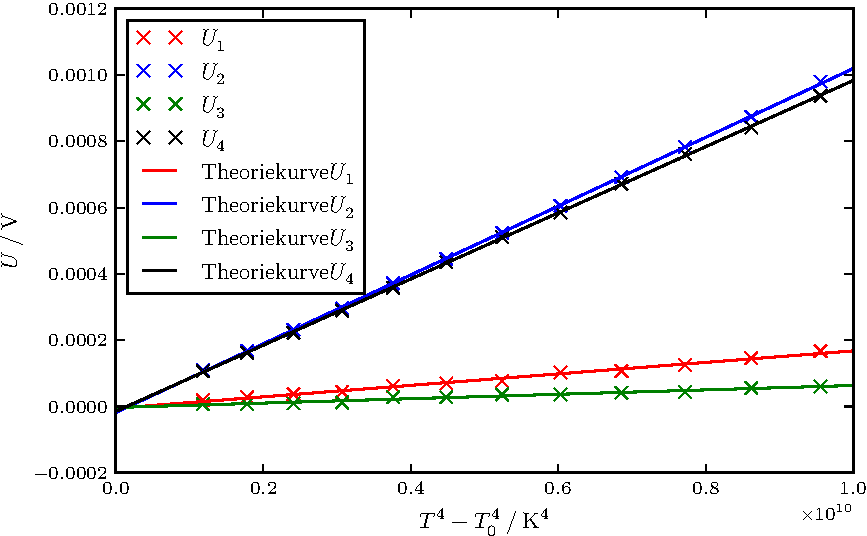
\includegraphics{build/plot.pdf}
%   \caption{Messdaten und Fitergebnis.}
%   \label{fig:plot}
% \end{figure}
%
% 2x2 Plot
% \begin{figure*}
%     \centering
%     \begin{subfigure}[b]{0.475\textwidth}
%         \centering
%         \includegraphics[width=\textwidth]{Abbildungen/Schaltung1.pdf}
%         \caption[]%
%         {{\small Schaltung 1.}}
%         \label{fig:Schaltung1}
%     \end{subfigure}
%     \hfill
%     \begin{subfigure}[b]{0.475\textwidth}
%         \centering
%         \includegraphics[width=\textwidth]{Abbildungen/Schaltung2.pdf}
%         \caption[]%
%         {{\small Schaltung 2.}}
%         \label{fig:Schaltung2}
%     \end{subfigure}
%     \vskip\baselineskip
%     \begin{subfigure}[b]{0.475\textwidth}
%         \centering
%         \includegraphics[width=\textwidth]{Abbildungen/Schaltung4.pdf}    % Zahlen vertauscht ... -.-
%         \caption[]%
%         {{\small Schaltung 3.}}
%         \label{fig:Schaltung3}
%     \end{subfigure}
%     \quad
%     \begin{subfigure}[b]{0.475\textwidth}
%         \centering
%         \includegraphics[width=\textwidth]{Abbildungen/Schaltung3.pdf}
%         \caption[]%
%         {{\small Schaltung 4.}}
%         \label{fig:Schaltung4}
%     \end{subfigure}
%     \caption[]
%     {Ersatzschaltbilder der verschiedenen Teilaufgaben.}
%     \label{fig:Schaltungen}
% \end{figure*}
